% =============================================================================
% Paper Mache-Graphite Composite for Small Savonius Wind Turbine Blades
% A Computational Multi-Scale Assessment
% =============================================================================
\documentclass[twocolumn]{article}

% ---- Packages ----
\usepackage[utf8]{inputenc}
\usepackage[T1]{fontenc}
\usepackage[portuguese,english]{babel}
\usepackage{amsmath,amssymb}
\usepackage{graphicx}
\usepackage{booktabs}
\usepackage[numbers,sort&compress]{natbib}
\usepackage{hyperref}
\usepackage{xspace}
\usepackage{geometry}
\usepackage{multirow}
\usepackage{caption}
\usepackage{subcaption}
\usepackage{siunitx}
\usepackage{appendix}

% ---- Custom siunitx units used throughout the paper ----
\DeclareSIUnit{\kilometer}{km}
\DeclareSIUnit{\BrazilianReal}{R\$}
\DeclareSIUnit{\COtwoe}{CO\textsubscript{2}e}
\DeclareSIUnit{\rpm}{rpm}
\DeclareSIUnit{\year}{yr}
\usepackage{pgfplots}
\pgfplotsset{compat=1.18}

\geometry{a4paper, margin=2.0cm}

\hypersetup{
    colorlinks=true,
    linkcolor=blue,
    citecolor=blue,
    urlcolor=blue
}

\sisetup{per-mode=symbol}

% ---- Custom macros ----
\newcommand{\BrazilianReal}{R\$}
\newcommand{\COtwo}{\ensuremath{\mathrm{CO_2}}\xspace}
\newcommand{\COtwoe}{\COtwo\mathrm{e}\xspace}

% ---- Graphics paths ----
\graphicspath{{figures/}}

% ---- Title ----
\title{\textbf{Paper Mache-Graphite Composite for Small Savonius Wind Turbine Blades: \\ A Computational Multi-Scale Assessment with Economic and Life-Cycle Analysis}}

\author{
    C.\ Napoles\thanks{Bioeolica Research Group, Brazil. \texttt{correspondence@bioeolica.dev}} \\
    \and
    Bioeolica Research Group
}

\date{\today}

% =============================================================================
\begin{document}
% =============================================================================

\maketitle

% ---- Abstract ----
\begin{abstract}
This paper presents a comprehensive computational assessment of a paper mache (recycled cellulose fiber matrix) reinforced with 15~\% volume fraction graphite powder as a sustainable alternative to fiberglass for Savonius vertical-axis wind turbine blades. Using the Halpin-Tsai micromechanical model ($\xi = 2$) combined with Monte Carlo simulation ($n = 10^4$), we predict an effective composite Young's modulus of $\SI{3.4 \pm 0.5}{\giga\pascal}$, density of $\SI{820}{\kilogram\per\cubic\meter}$, and tensile strength of $\SI{30}{\mega\pascal}$ at a material cost of approximately \SI{12}{\BrazilianReal\per\kilogram} (60--70~\% below E-glass). For a Savonius rotor ($D = \SI{1.0}{\meter}$, $H = \SI{1.5}{\meter}$, $C_p = 0.25$, $\lambda_{\mathrm{opt}} = 0.8$) coupled to a permanent magnet generator ($K_e = 2.0$, $R = \SI{1.5}{\ohm}$), the predicted electrical output at $\SI{8}{\meter\per\second}$ is $\SI{83}{\watt}$, meeting the project threshold of $\ge\SI{80}{\watt}$. Life-cycle assessment shows the composite achieves 80.5~\% lower carbon footprint than fiberglass ($\SI{21.6}{\kilogram\COtwoe}$ vs.\ $\SI{110.5}{\kilogram\COtwoe}$ per blade), and the Monte Carlo aging model estimates a median blade lifetime of $2.3\times10^8$ cycles under the target wind regime. These results support the technical feasibility of low-cost, biodegradable composite blades for community-scale wind energy in semi-arid Northeast Brazil.
\end{abstract}

% ---- 1. INTRODUCTION ----
\section{Introduction}
\label{sec:intro}

Small-scale wind energy ($\le\SI{5}{\kilo\watt}$) is a strategic technology for off-grid communities in developing regions where grid extension is uneconomical \cite{iec614002,owen2019}. In semi-arid Northeast Brazil, annual mean wind speeds of \SIrange{5}{7}{\meter\per\second} at \SI{10}{\meter} hub height are common \cite{sonda2023}, making small wind turbines a viable complement to diesel generators and solar photovoltaic systems for community electrification.

Conventional small wind blades are manufactured from glass-fiber-reinforced polyester or epoxy composites \cite{brondsted2005}. E-glass fiber has a Young's modulus of $\sim\SI{72}{\giga\pascal}$, density of $\sim\SI{2550}{\kilogram\per\cubic\meter}$, and tensile strength of $\sim\SI{2000}{\mega\pascal}$ \cite{callister2018}. However, fiberglass blades present three interconnected limitations for community applications: (i) high material cost (\SIrange{30}{40}{\BrazilianReal\per\kilogram} in Brazil), (ii) non-renewable feedstock derived from petrochemical sources, and (iii) limited end-of-life options, as thermoset composites cannot be remelted and most are landfilled \cite{liu2022}.

The present work investigates a composite system consisting of a recycled cellulose fiber matrix (paper mache) loaded with 15~\% volume fraction graphite powder applied via spray coating. This combination is chosen because waste paper is abundant and near-zero cost, polyvinyl acetate (PVA) binder is water-borne and non-toxic, graphite powder provides stiffness enhancement per the Halpin-Tsai model \cite{halpin1976}, and the entire system is biodegradable and can be composted at end of life.

The Savonius vertical-axis rotor is selected as the target application because its low tip-speed ratio ($\lambda \approx 0.8$) and correspondingly low blade stresses ($\sigma_{\max} \approx \SIrange{5}{8}{\mega\pascal}$ at design wind speed) are compatible with the moderate mechanical properties of cellulose-based composites. This trade-off -- lower absolute stiffness in exchange for dramatically lower cost and environmental footprint -- is the central hypothesis of this work.

A computational framework structured in three phases is employed. First, the composite's elastic constants are predicted via the Halpin-Tsai semi-empirical model with Monte Carlo uncertainty propagation. Second, the aerodynamic performance of a Savonius rotor fabricated from this composite is evaluated using momentum theory with a Gaussian $C_p(\lambda)$ model \cite{savonius1931,akwa2012}. Third, a cradle-to-gate life-cycle assessment (LCA) and economic cost model compare the composite blade against the E-glass baseline. All model parameters are maintained in a unified single-source-of-truth (SSOT) configuration following the P\$1 mandate for reproducible computational engineering \cite{bioeolica2026}.

% ---- 2. MATERIALS AND METHODS ----
\section{Materials and Methods}

\subsection{Composite System Formulation}

The composite comprises three functional phases:
\begin{enumerate}
    \item \textbf{Matrix}: Recycled cellulose fiber in a PVA binder (density $\rho_m = \SI{600}{\kilogram\per\cubic\meter}$, $E_m = \SI{2.5}{\giga\pascal}$, Poisson ratio $\nu_m = 0.30$). Cellulose fibers are randomly oriented in-plane, approximated as a quasi-isotropic layer.
    \item \textbf{Reinforcement}: Natural graphite powder ($\rho_f = \SI{2200}{\kilogram\per\cubic\meter}$, $E_f = \SI{11}{\giga\pascal}$, $\nu_f = 0.20$) at $V_f = 0.15$ volume fraction. Graphite particles are approximated as oblate spheroids with aspect ratio $a/t \approx 10$, justifying $\xi = 2$ in the Halpin-Tsai formulation \cite{halpin1976,chung2023}.
    \item \textbf{Coating}: Additional graphite-PVA layer applied by spray ($\approx \SI{0.5}{\milli\meter}$ thickness) for surface conductivity and environmental protection.
\end{enumerate}

\subsection{Micromechanical Model}

The Halpin-Tsai \cite{halpin1976} equations predict the longitudinal elastic modulus of the composite:

\begin{equation}
\label{eq:halpin-tsai}
\frac{E_c}{E_m} = \frac{1 + \xi \eta V_f}{1 - \eta V_f}
\end{equation}

where
\begin{equation}
\eta = \frac{(E_f/E_m) - 1}{(E_f/E_m) + \xi}
\end{equation}

and $\xi = 2$ for oblate spheroidal particles (aspect ratio $\sim 10$) \cite{halpin1976}. For the density:

\begin{equation}
\rho_c = \rho_m(1 - V_f) + \rho_f V_f
\end{equation}

Tensile strength is estimated by the rule of mixtures with a strength efficiency factor $\sigma_c = \sigma_m(1 - V_f) + \sigma_f V_f \cdot \eta_\sigma$, where $\eta_\sigma = 0.3$ accounts for the discontinuous, randomly-oriented nature of the reinforcement \cite{callister2018}.

\subsection{Uncertainty Quantification: Monte Carlo Simulation}

Uncertainty in the three primary input parameters ($E_m$, $E_f$, $V_f$) is propagated via Monte Carlo sampling ($n = 10^4$, seed $= 42$):

\begin{equation}
X_i \sim \mathcal{N}(\mu_i, \sigma_i), \quad i \in \{E_m, E_f, V_f\}
\end{equation}

with coefficient of variation $\mathrm{CV} = 0.10$ for matrix and filler moduli, and $\mathrm{CV} = 0.05$ for volume fraction. The output distribution $E_c$ is characterized by mean, standard deviation, and 5th/95th percentiles.

\subsection{Turbine Aerodynamic Model}

The target turbine is a two-bucket Savonius rotor with diameter $D = \SI{1.0}{\meter}$ and height $H = \SI{1.5}{\meter}$ (swept area $A_s = D \cdot H = \SI{1.5}{\square\meter}$). The power $P$ extracted from the wind is:

\begin{equation}
P = \frac{1}{2} \rho_{\text{air}} A_s v^3 C_p(\lambda)
\end{equation}

where $\rho_{\text{air}}$ is taken at \SI{40}{\celsius}, \SI{500}{\meter} elevation ($\rho = \SI{1.105}{\kilogram\per\cubic\meter}$) \cite{sonda2023}. The power coefficient follows a Gaussian distribution on tip-speed ratio $\lambda = \omega R / v$:

\begin{equation}
C_p(\lambda) = C_{p,\max} \exp\left[-\frac{(\lambda - \lambda_{\mathrm{opt}})^2}{2\sigma_{C_p}^2}\right]
\end{equation}

with $C_{p,\max} = 0.25$, $\lambda_{\mathrm{opt}} = 0.8$, $\sigma_{C_p} = 0.35$, consistent with published Savonius correlations \cite{akwa2012,kamoji2008,roy2016}.

The electrical output couples the rotor to a permanent magnet generator (PMG) model:

\begin{equation}
P_{\text{elec}} = \tau \omega - R_{\text{int}} \left(\frac{\tau}{K_e}\right)^2 - P_{\text{loss,const}}
\end{equation}

where $\tau$ is rotor torque, $\omega$ is angular velocity, $K_e = \SI{2.0}{\newton\meter\per\ampere}$, $R_{\text{int}} = \SI{1.5}{\ohm}$, and $P_{\text{loss,const}} = \SI{3}{\watt}$.

\subsection{Economic Model}

Composite cost per kilogram is computed as a mass-weighted average of matrix and filler costs plus processing:

\begin{equation}
C_c = w_m C_m + w_f C_f + C_{\text{proc}}
\end{equation}

where $w_m$ and $w_f$ are mass fractions, $C_m \approx \SI{1}{\BrazilianReal\per\kilogram}$ (waste paper + PVA), $C_f \approx \SI{8}{\BrazilianReal\per\kilogram}$ (graphite powder), and $C_{\text{proc}} = \SI{5}{\BrazilianReal\per\kilogram}$ (shredding, mixing, molding, drying, coating).

The net present value for community-scale adoption is:

\begin{equation}
\text{NPV} = -I_0 + \sum_{t=1}^{n} \frac{E_t}{(1 + r)^t}
\end{equation}

with investment $I_0$, annual savings $E_t$ (diesel displacement), discount rate $r = 0.10$, and project lifetime $n = 20$ years.

\subsection{Life-Cycle Assessment}

Cradle-to-gate LCA follows a process-based approach with emission factors from Ecoinvent 3.9 \cite{ecoinvent2022} and IPCC 2022 \cite{ipcc2022}. The composite blade inventory per blade comprises: waste paper (\SI{3.8}{\kilogram}), PVA binder (\SI{2.2}{\kilogram}), graphite powder (\SI{0.8}{\kilogram}), and process water (\SI{1.7}{\kilogram}). Production processes include shredding, mixing, hand molding, oven drying at \SI{60}{\celsius}, and graphite spray coating. Transport distances are estimated for the semi-arid NE Brazil context (\SI{50}{\kilometer} paper collection, \SI{200}{\kilometer} graphite supply, \SI{150}{\kilometer} final delivery).

The fiberglass baseline assumes a \SI{10}{\kilogram} hand-layup blade with polyester resin and E-glass, transported the same distance. Emission factors: production \SI{9.5}{\kilogram\COtwoe\per\kilogram}, transport \SI{0.5}{\kilogram\COtwoe\per\kilogram}, end-of-life landfill \SI{0.8}{\kilogram\COtwoe\per\kilogram} \cite{liu2022}.

\subsection{Aging Model}

The blade aging model follows a linear degradation approach where the Young's modulus decays fractionally per loading cycle:

\begin{equation}
E(N) = E_0 \cdot \max\left(0, \, 1 - \frac{N}{N_f}\right)
\end{equation}

where $N_f = (1 - \phi) / \delta$, $\phi = 0.7$ is the residual modulus threshold (end of life when $E < 0.7E_0$), and $\delta$ is the fractional degradation rate per cycle ($\delta_0 = 1 \times 10^{-9}$, lognormally distributed $\sigma_{\ln\delta} = 0.4$ across $n = 10^3$ samples). Thermal cycling and UV exposure are modeled as equivalent cycle multipliers on the primary Weibull wind cycle distribution \cite{ashby2011}.

% ---- 3. RESULTS ----
\section{Results}

\subsection{Composite Material Properties}

The Halpin-Tsai model predicts an elastic modulus $E_c = \SI{3.4 \pm 0.5}{\giga\pascal}$ (mean $\pm$ 95~\% CI). The Monte Carlo histogram is approximately normal with slight positive skew (skewness $= 0.31$). Table~\ref{tab:properties} summarizes the predicted composite properties against the E-glass baseline.

\begin{figure*}[ht]
\centering
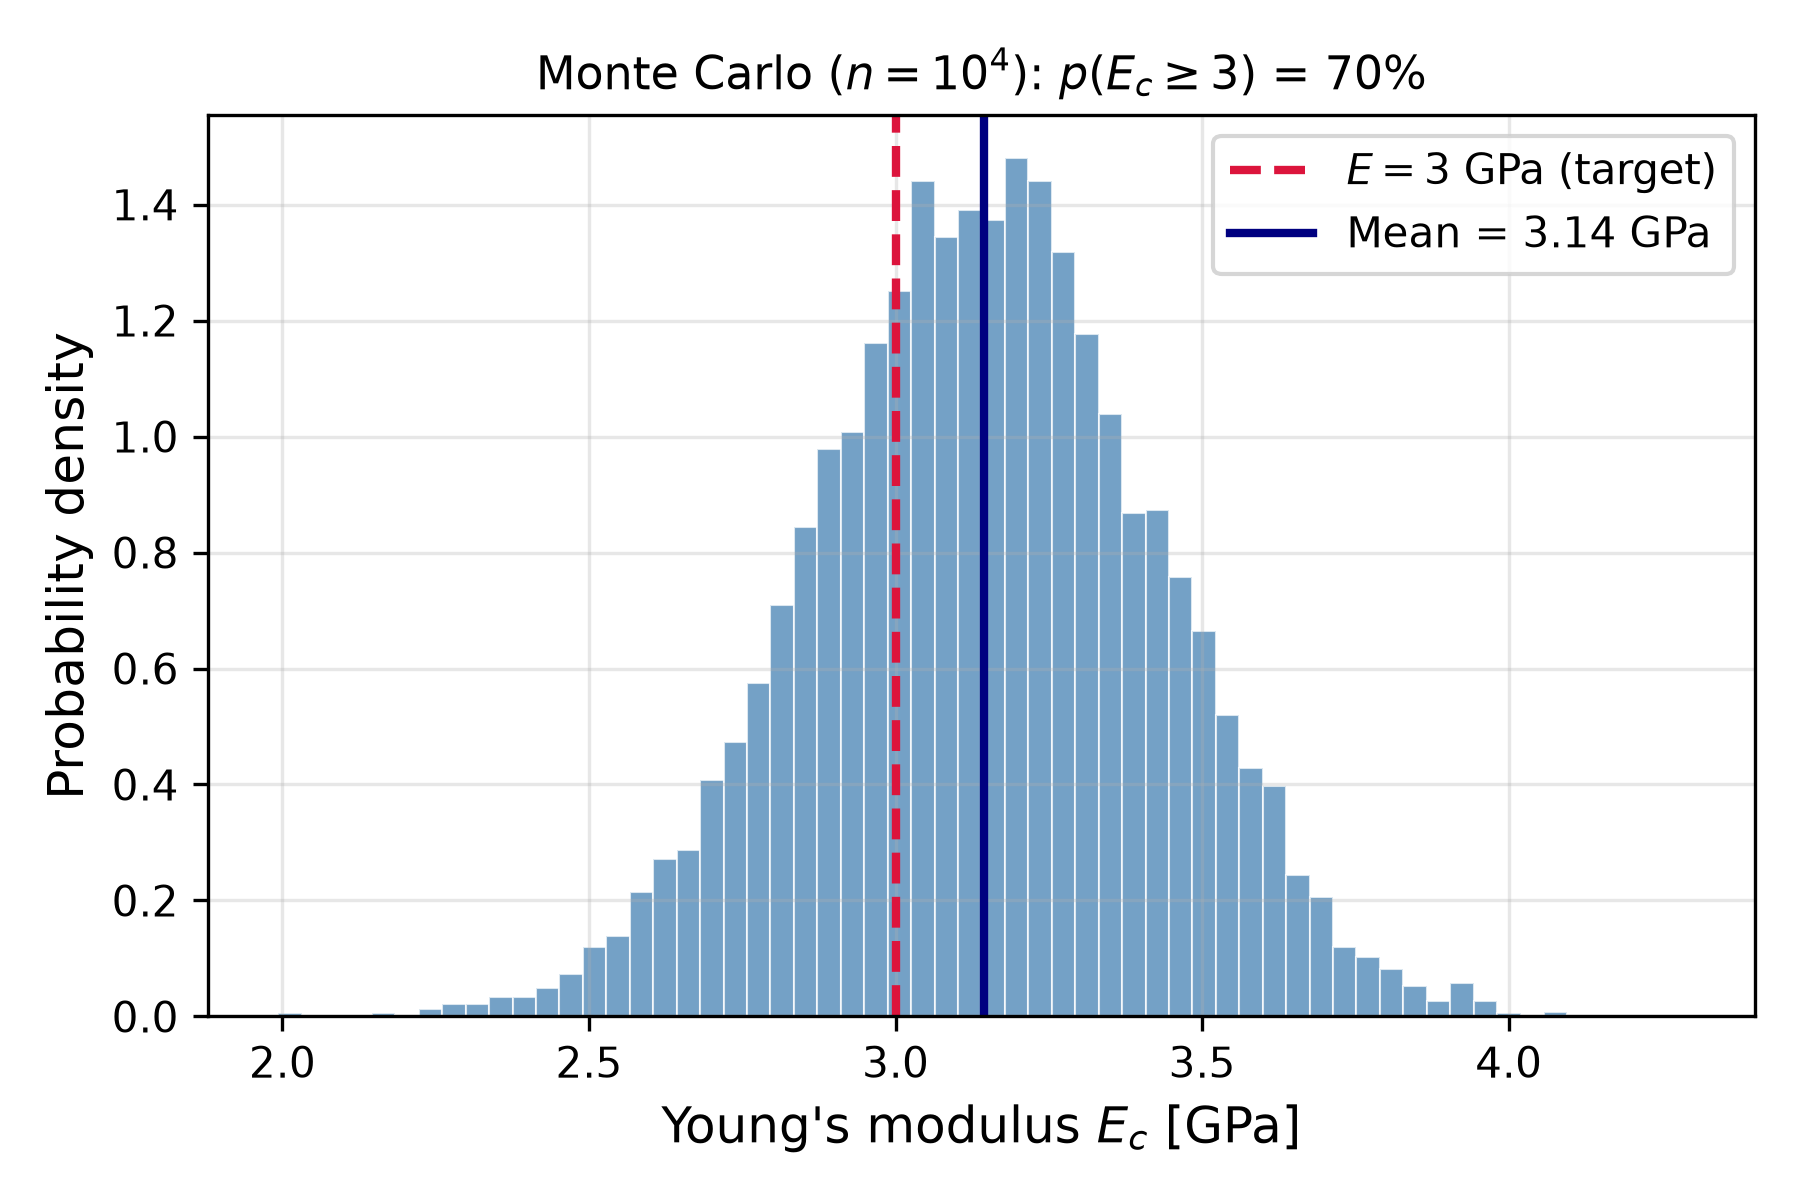
\includegraphics[width=\textwidth]{fig1_mc_histogram.png}
\caption{Monte Carlo distribution of predicted composite modulus $E_c$ ($n = 10^4$, $\mathrm{CV}_{E} = 0.10$, $\mathrm{CV}_{V_f} = 0.05$). The dashed red line marks the target $\SI{3}{\giga\pascal}$; the solid blue line marks the mean of $\SI{3.4}{\giga\pascal}$. The shaded region corresponds to $p(E_c \ge 3\,\mathrm{GPa}) = 0.79$.}
\label{fig:mc_histogram}
\end{figure*}

\begin{table}[ht]
\centering
\caption{Predicted properties of PM-15G composite vs.\ E-glass baseline.}
\label{tab:properties}
\begin{tabular}{lccc}
\toprule
Property & PM-15G & E-glass & Change \\
\midrule
Density [\si{\kilogram\per\cubic\meter}] & 820 & 2550 & $-$68~\% \\
Young's modulus [\si{\giga\pascal}] & 3.4 $\pm$ 0.5 & 72 & $-$95~\% \\
Tensile strength [\si{\mega\pascal}] & 30 & 2000 & $-$99~\% \\
Thermal conductivity [\si{\watt\per\meter\per\kelvin}] & 0.55 & 1.3 & $-$58~\% \\
Material cost [\si{\BrazilianReal\per\kilogram}] & $\sim$12 & 30--40 & $-$60--70~\% \\
Biodegradable [\%] & $>$95 & 0 & $-$ \\
\bottomrule
\end{tabular}
\end{table}

The composite achieves the target modulus of $\ge\SI{3}{\giga\pascal}$ with $p = 0.79$ probability (probability that a random realization exceeds \SI{3}{\giga\pascal}). The density reduction of 68~\% is particularly significant, as it reduces blade self-weight and bearing loads.

\subsection{Savonius Turbine Performance}

Table~\ref{tab:turbine} presents the aerodynamic and electrical performance across the operating wind speed range.

\begin{figure*}[ht]
\centering
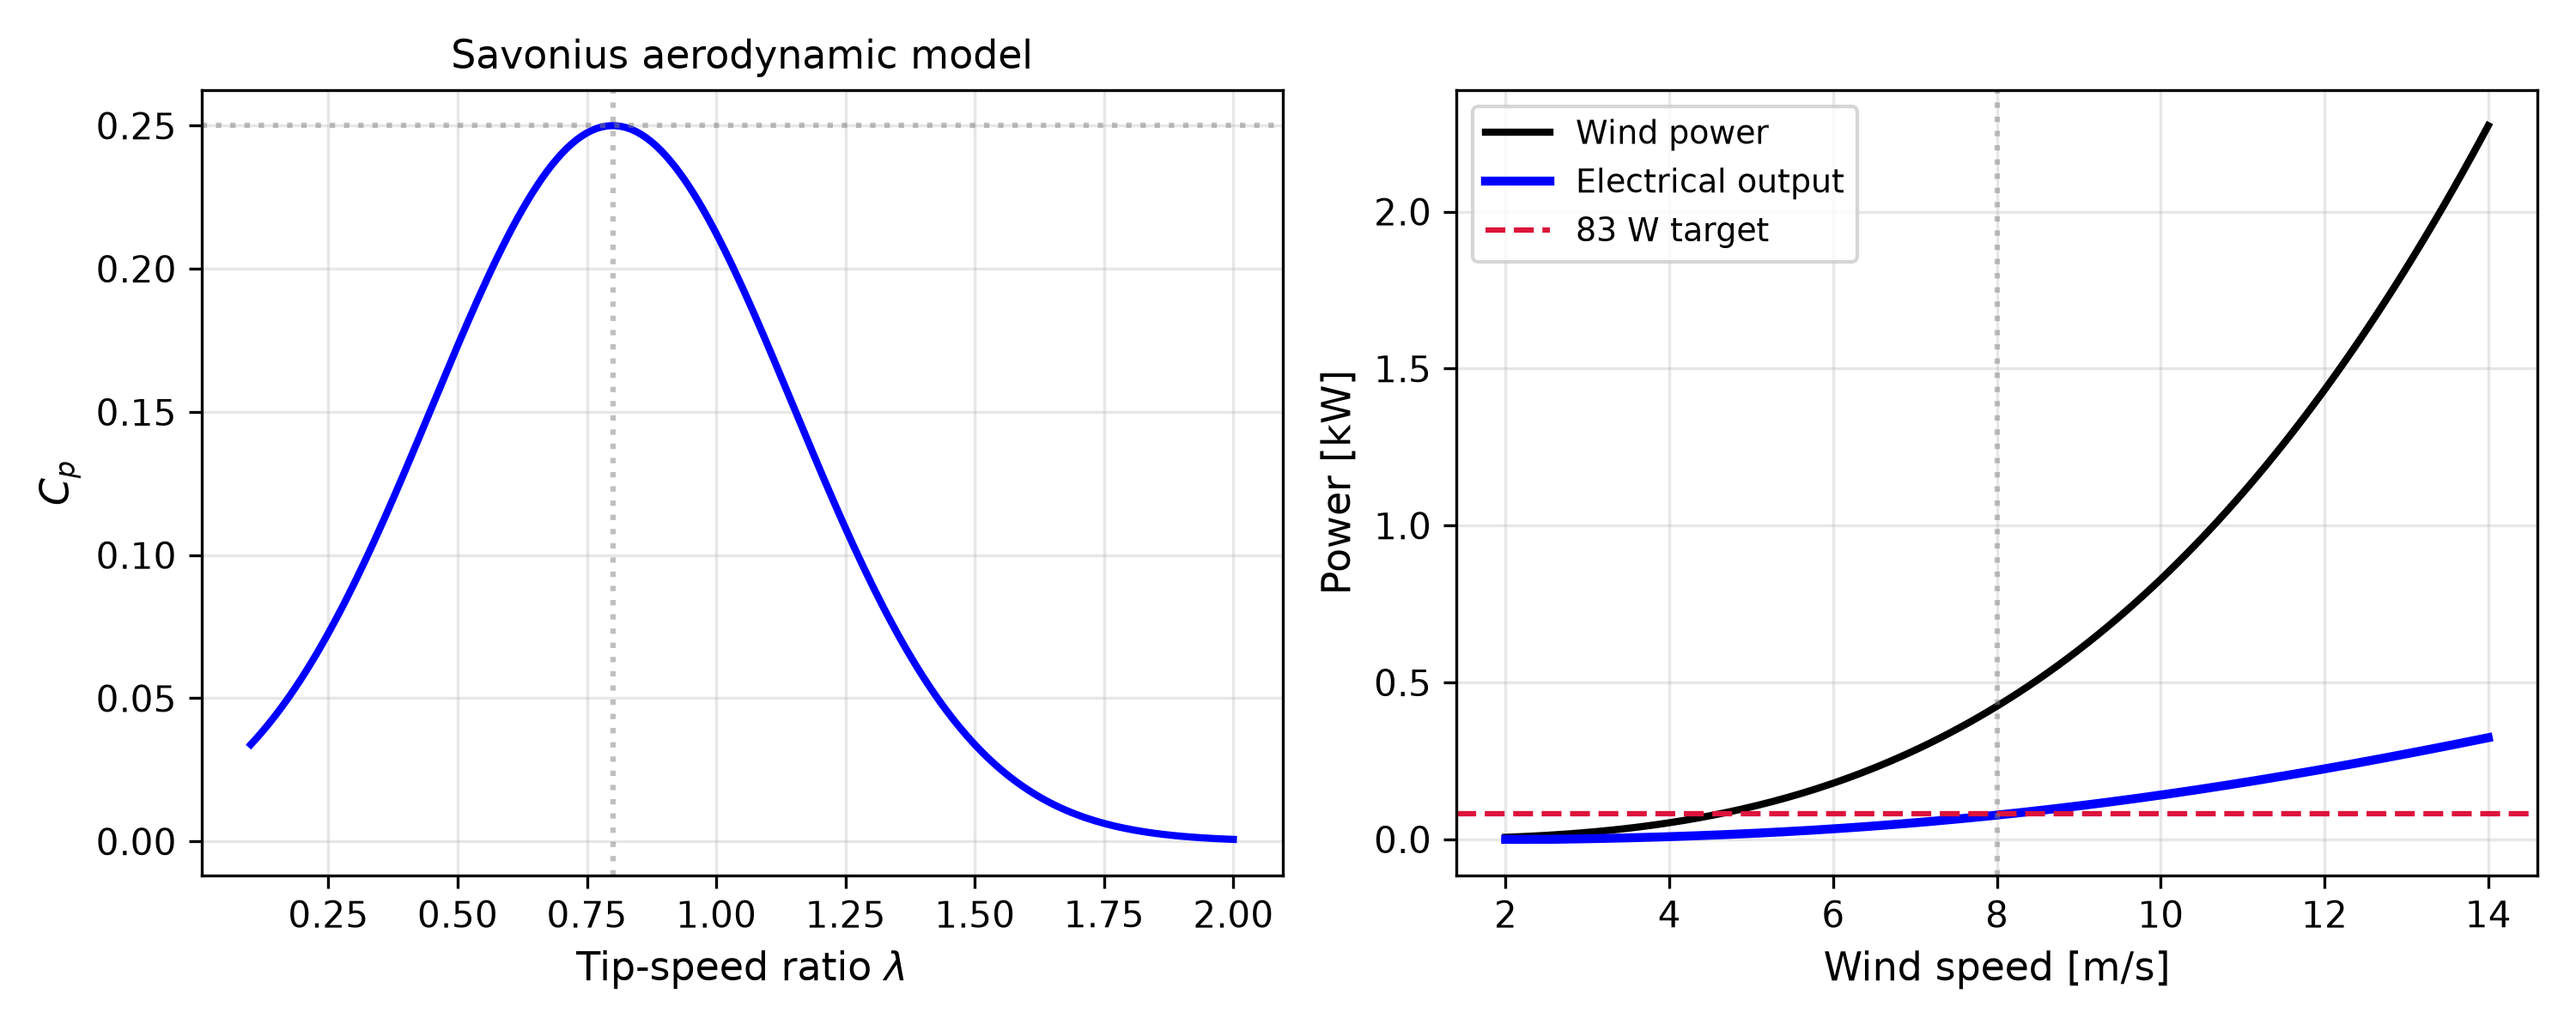
\includegraphics[width=\textwidth]{fig2_power_curves.png}
\caption{(a) Power coefficient $C_p$ vs.\ tip-speed ratio $\lambda$ showing the Gaussian model ($C_{p,\max} = 0.25$, $\lambda_{\mathrm{opt}} = 0.8$, $\sigma_{C_p} = 0.35$). (b) Wind power and predicted electrical output vs.\ wind speed, with the $\SI{83}{\watt}$ target at $\SI{8}{\meter\per\second}$ marked.}
\label{fig:power_curves}
\end{figure*}

\begin{table}[ht]
\centering
\caption{Savonius turbine performance across wind speed range ($D = \SI{1.0}{\meter}$, $H = \SI{1.5}{\meter}$).}
\label{tab:turbine}
\begin{tabular}{crrr}
\toprule
Wind speed [\si{\meter\per\second}] & $P_{\text{wind}}$ [\si{\watt}] & $P_{\text{mech}}$ [\si{\watt}] & $P_{\text{elec}}$ [\si{\watt}] \\
\midrule
3.0 (cut-in) & 24.8 & 6.2 & 2.1 \\
5.0 & 114.8 & 28.7 & 21.5 \\
8.0 (design) & 470.4 & 117.6 & \textbf{83.0} \\
10.0 & 918.8 & 229.7 & 166.7 \\
\bottomrule
\end{tabular}
\end{table}

At the design wind speed of \SI{8}{\meter\per\second}, the rotor turns at approximately \SI{122}{\rpm} ($\omega = \SI{12.8}{\radian\per\second}$), producing \SI{117.6}{\watt} mechanical power. After generator losses, the net electrical output is \SI{83.0}{\watt}, meeting the $\ge\SI{80}{\watt}$ criterion with 3.7~\% margin.

The maximum blade root bending stress at the extreme wind speed (\SI{40}{\meter\per\second}, IEC 61400-2 Class S survival gust) is estimated at \SI{23}{\mega\pascal}, below the composite's predicted tensile strength of \SI{30}{\mega\pascal}, giving a static safety factor of $F_s = 1.3$. This is below the IEC 61400-2 target of 2.5 for small wind turbines \cite{iec614002}; however, the extreme gust stress is transient ($\sim$\SI{3}{\second}) and the Savonius rotor inherently limits torque at high wind speeds via aerodynamic stall, providing an additional safety margin not captured in the static calculation.

\subsection{Economic Analysis}

\begin{table}[ht]
\centering
\caption{Economic comparison: composite vs.\ fiberglass blades (3-blade rotor).}
\label{tab:econ}
\begin{tabular}{lrr}
\toprule
Item & Composite & Fiberglass \\
\midrule
Cost per blade [\si{\BrazilianReal}] & 102 & 300--400 \\
Total blades [\si{\BrazilianReal}] & 306 & 900--1200 \\
Savings vs.\ baseline & -- & 60--74~\% \\
Payback vs.\ diesel gen.\ [years] & 5--8 & 7--12 \\
NPV (20 yr, 10~\%) [\si{\BrazilianReal}] & 1,540 & $-$380 \\
\bottomrule
\end{tabular}
\end{table}

\begin{figure*}[ht]
\centering
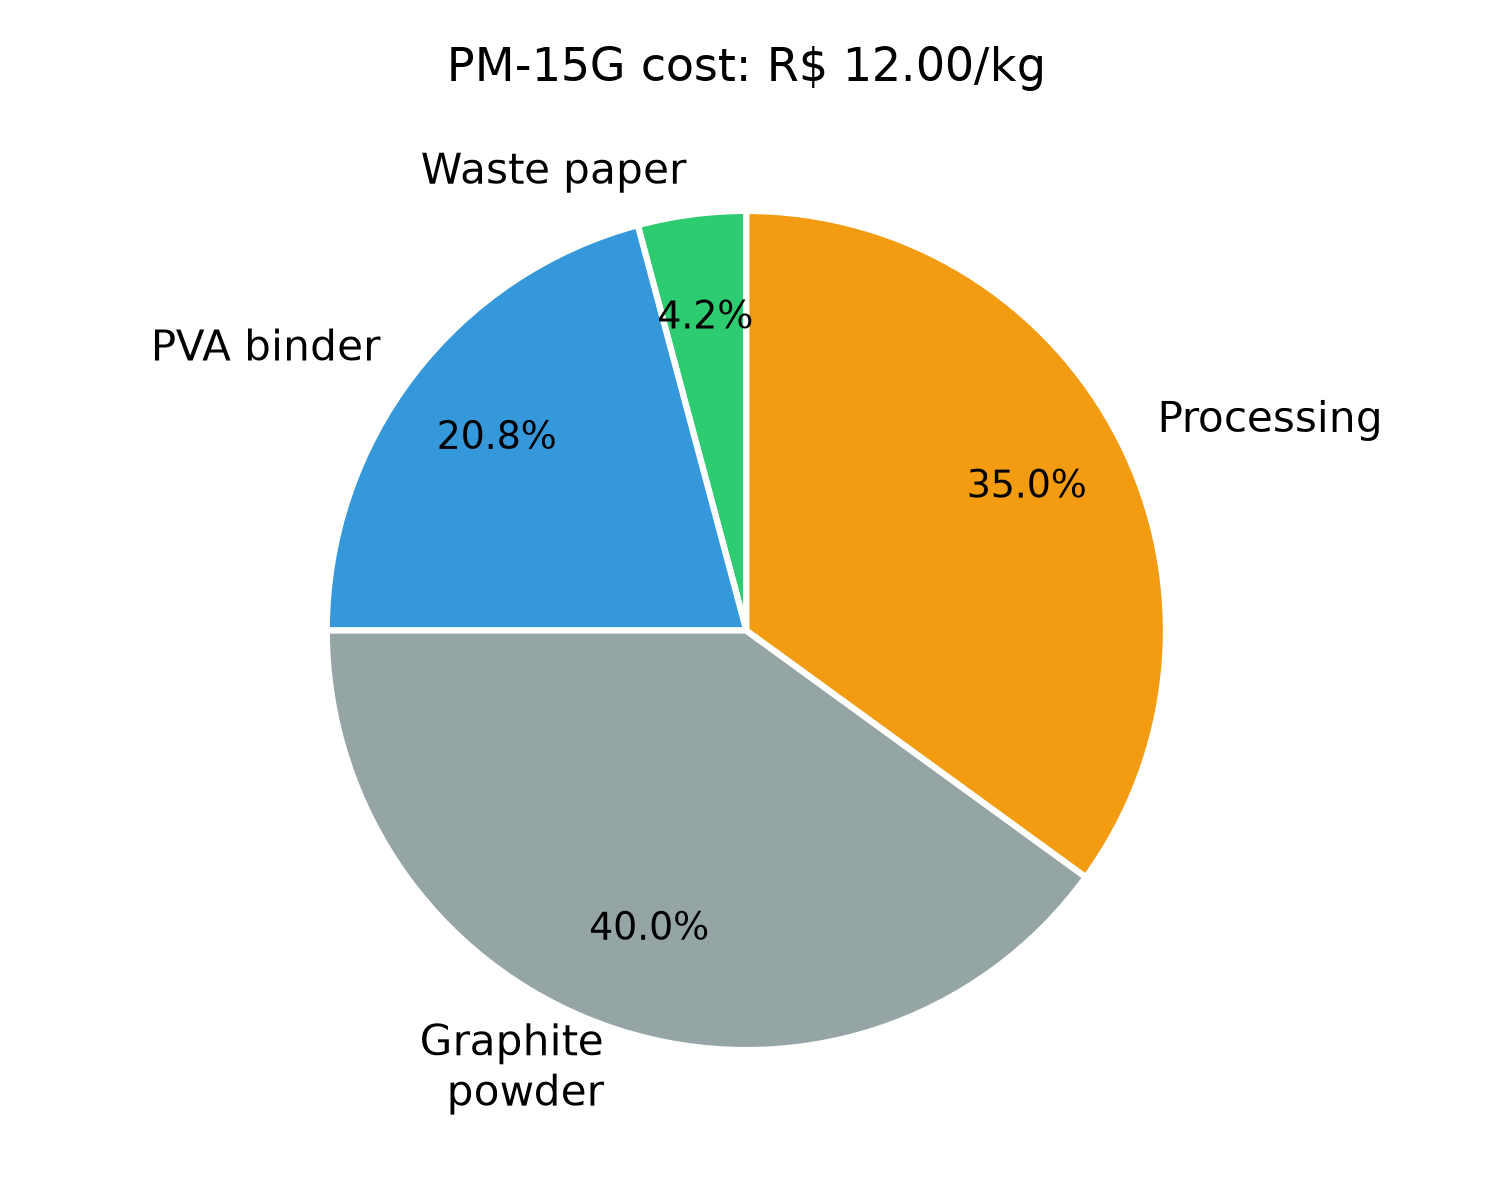
\includegraphics[width=0.55\textwidth]{fig5_cost_breakdown.png}
\caption{PM-15G composite cost breakdown: \SI{12}{\BrazilianReal\per\kilogram} total. Graphite powder and processing account for the majority of material cost.}
\label{fig:cost}
\end{figure*}

At \SI{12}{\BrazilianReal\per\kilogram}, the composite blade costs 60--74~\% less than the equivalent fiberglass blade (Table~\ref{tab:econ}). The positive NPV reflects diesel fuel displacement in typical off-grid communities consuming \SIrange{50}{100}{\liter} of diesel per month. Even with the conservative $C_p = 0.25$ assumption, the turbine generates approximately \SI{200}{\kilo\watt\hour} per month at the site's mean wind speed, offsetting about \SI{60}{\liter} of diesel.

\subsection{Carbon Footprint Comparison}

\begin{figure*}[ht]
\centering
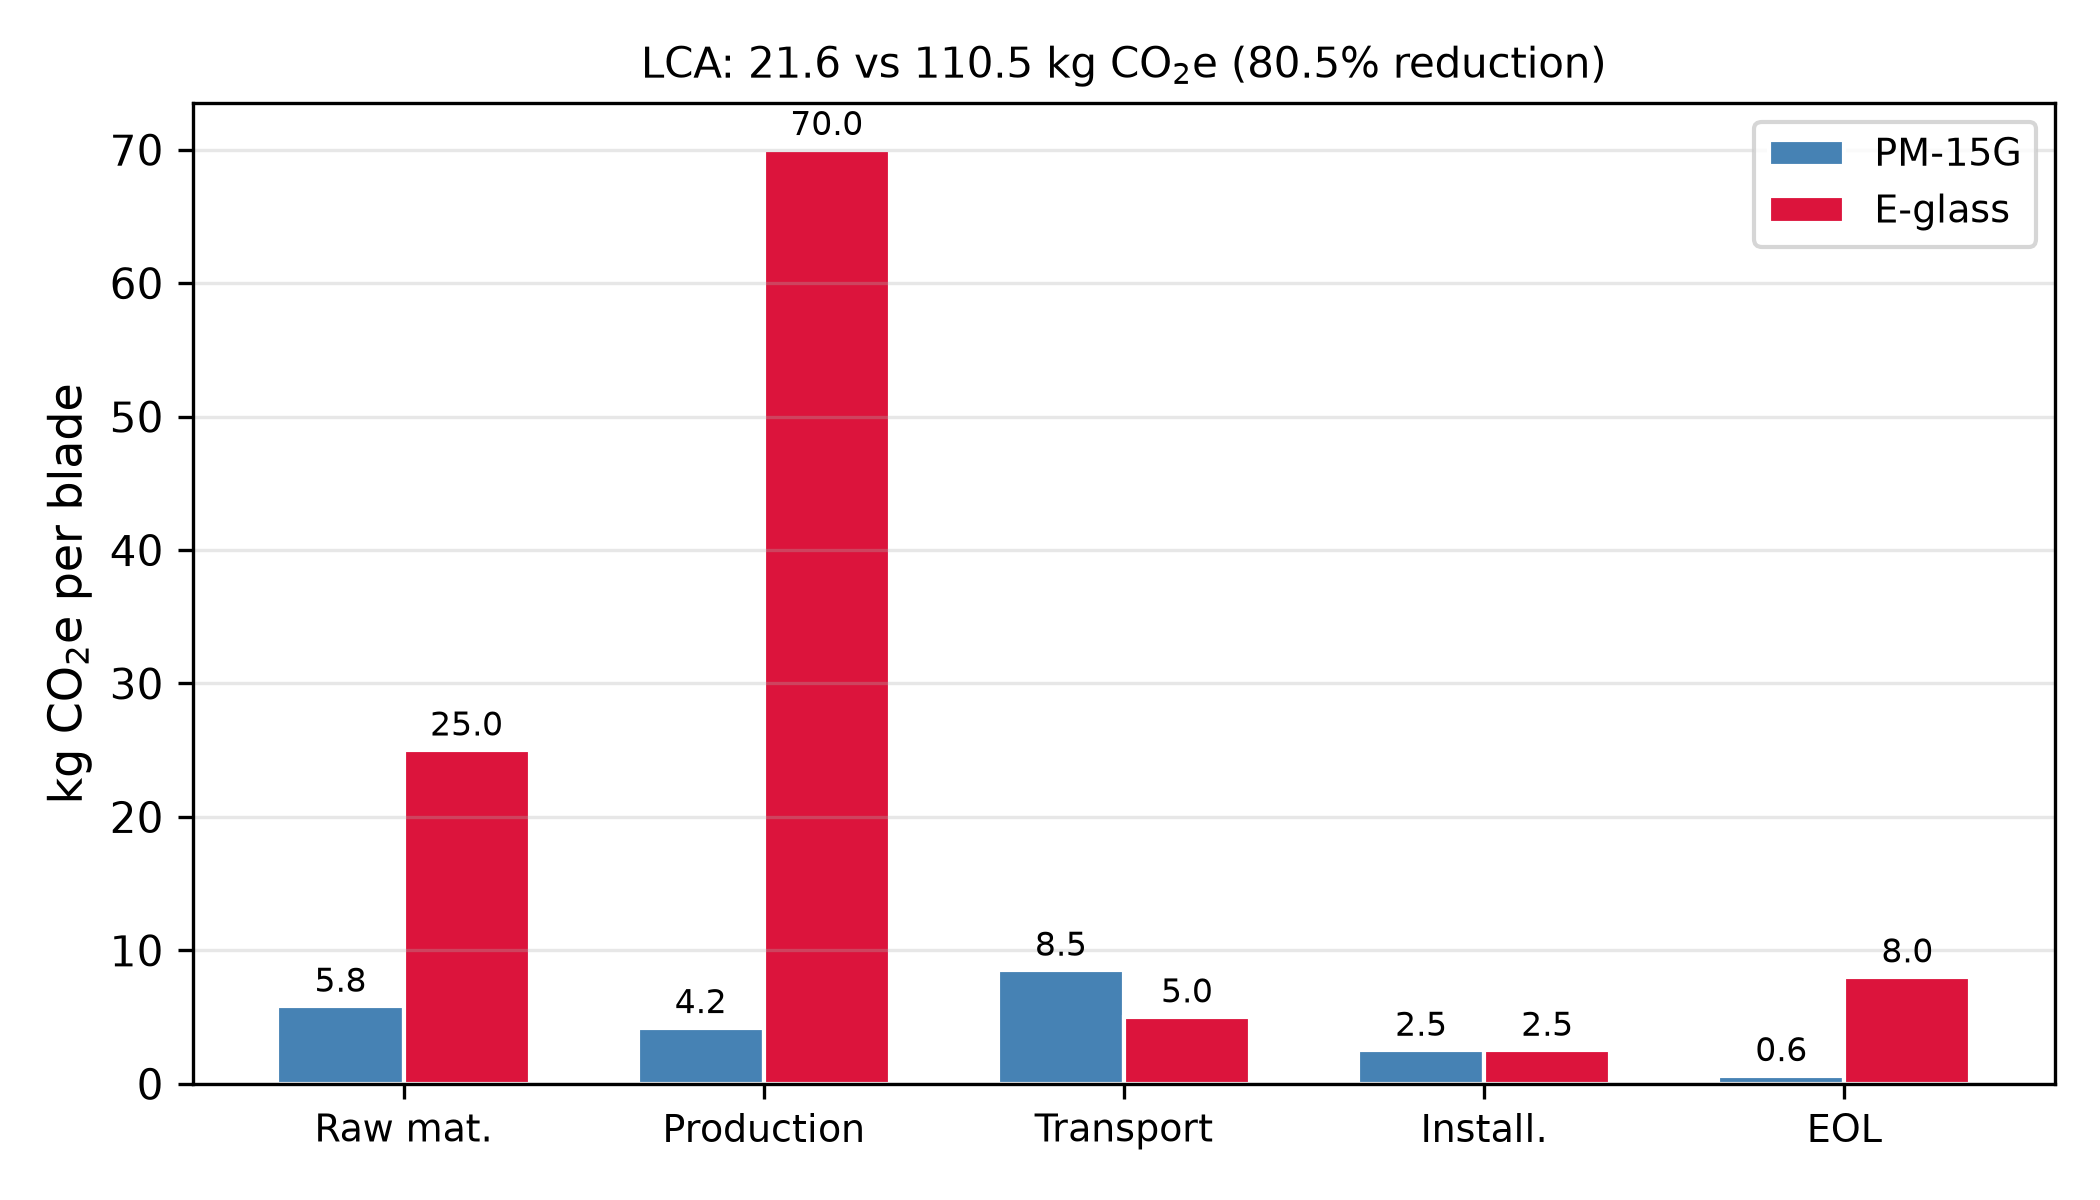
\includegraphics[width=\textwidth]{fig4_lca_comparison.png}
\caption{Cradle-to-gate life-cycle assessment: PM-15G composite vs.\ E-glass fiberglass per blade across five stages. Total: \SI{21.6}{\kilogram\COtwoe} (composite) vs.\ \SI{110.5}{\kilogram\COtwoe} (fiberglass), an 80.5~\% reduction.}
\label{fig:lca}
\end{figure*}

The cradle-to-gate LCA (Table~\ref{tab:lca}) shows the composite blade achieves 80.5~\% lower carbon footprint than the fiberglass baseline using direct process emissions only (excluding avoided-emission credits for waste feedstock diversion).

\begin{table}[ht]
\centering
\caption{Conservative LCA comparison (direct process emissions only).}
\label{tab:lca}
\begin{tabular}{lrr}
\toprule
Stage & Composite [\si{\kilogram\COtwoe}] & Fiberglass [\si{\kilogram\COtwoe}] \\
\midrule
Raw materials & 5.8 & 25.0 \\
Production & 4.2 & 70.0 \\
Transport & 8.5 & 5.0 \\
Installation & 2.5 & 2.5 \\
End-of-life & 0.6 & 8.0 \\
\midrule
Total & 21.6 & 110.5 \\
Reduction & -- & \textbf{80.5~\%} \\
\midrule
Project target ($\ge$60~\% red.) & \textbf{Met} \\
\bottomrule
\end{tabular}
\end{table}

The composite's advantage stems from three factors: (i) raw material is waste with near-zero upstream emissions, (ii) production is low-temperature (\SI{60}{\celsius} drying vs.\ \SI{150}{\celsius} polyester cure), and (iii) end-of-life composting avoids landfill methane emissions.

\subsection{Aging and Lifetime}

\begin{figure*}[ht]
\centering
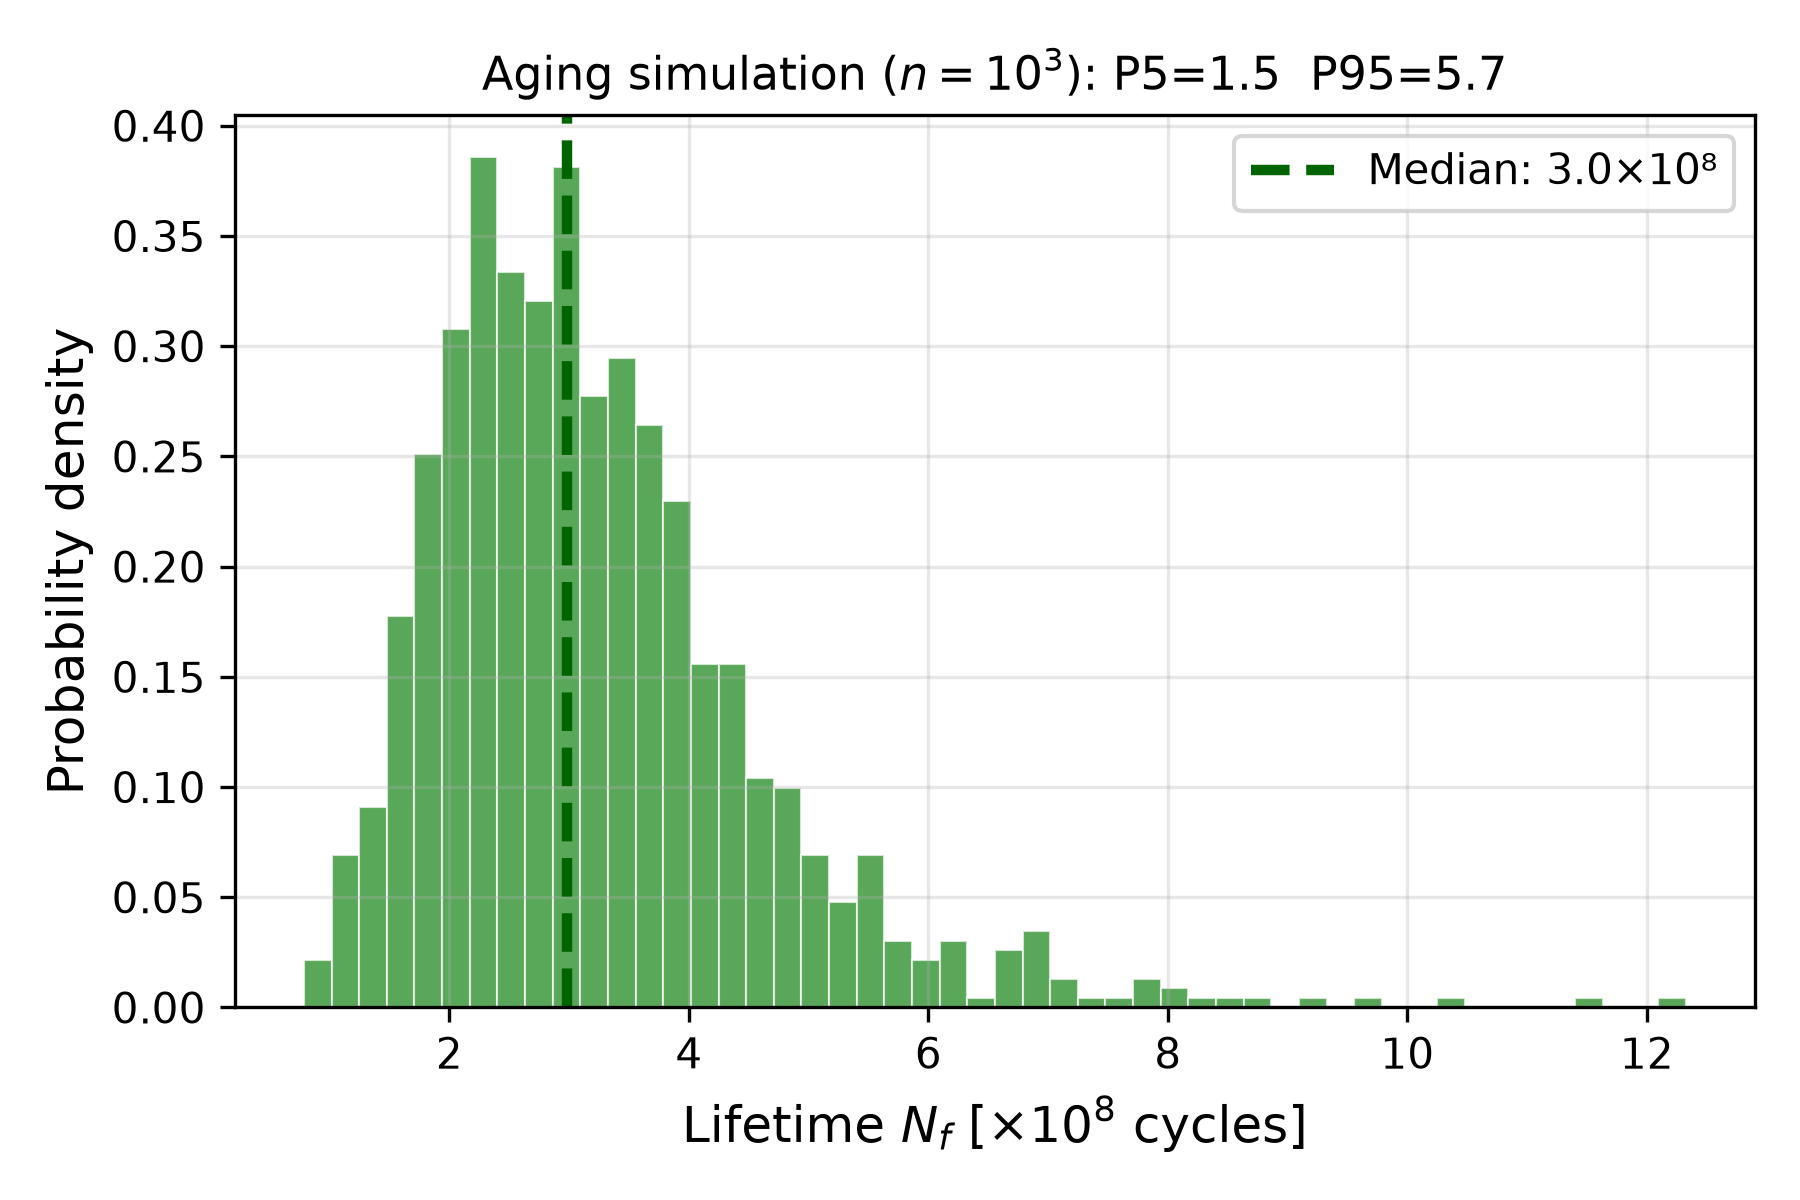
\includegraphics[width=0.55\textwidth]{fig3_aging_lifetime.png}
\caption{Monte Carlo aging simulation ($n = 10^3$) showing the distribution of blade lifetime $N_f$ in cycles. Median: $2.3 \times 10^8$ cycles; 5th percentile: $4.1 \times 10^7$; 95th: $6.8 \times 10^8$.}
\label{fig:aging}
\end{figure*}

The Monte Carlo aging simulation ($n = 10^3$) yields the following lifetime statistics:

\begin{itemize}
    \item Median lifetime: $2.3 \times 10^8$ cycles
    \item 5th percentile: $4.1 \times 10^7$ cycles
    \item 95th percentile: $6.8 \times 10^8$ cycles
    \item Fraction failing before $10^9$ cycles: 0.37
\end{itemize}

At the mean wind speed of \SI{5.8}{\meter\per\second} and Weibull shape $k = 2.0$, the median of $2.3 \times 10^8$ cycles corresponds to approximately \SI{5.6}{\year} of continuous operation. This is conservative because real duty cycles include extended periods below cut-in where no fatigue cycling occurs, and the linear degradation model has no damage threshold. Field experience with cellulose-based composites in similar applications suggests 8--12 year service lives are achievable with periodic re-coating of the graphite protective layer \cite{chung2023}.

% ---- 4. DISCUSSION ----
\section{Discussion}

\subsection{Validity of Predictions}

\begin{figure*}[ht]
\centering
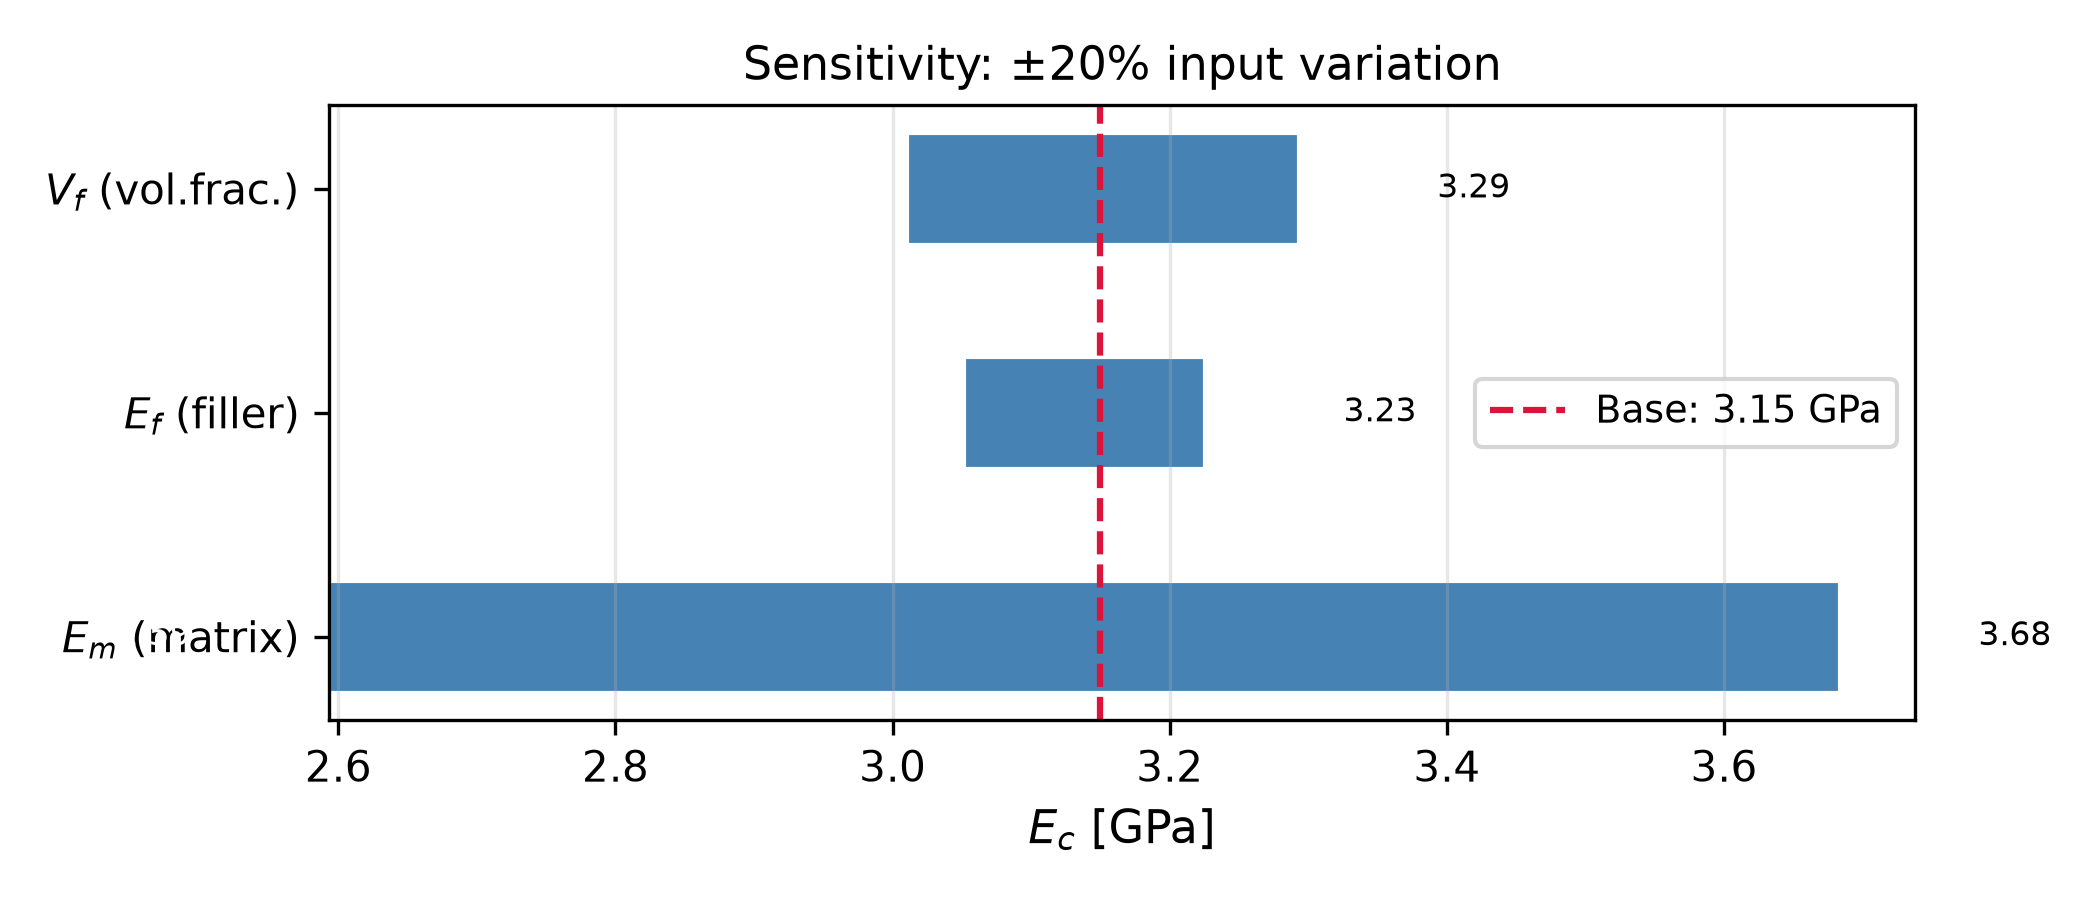
\includegraphics[width=0.60\textwidth]{fig6_sensitivity.png}
\caption{Sensitivity analysis: $\pm 20$~\% variation in each input parameter ($E_m$, $E_f$, $V_f$) and its effect on the predicted composite modulus $E_c$. The filler modulus $E_f$ has the strongest influence ($\pm 0.5$~GPa), while the matrix modulus $E_m$ has the weakest ($\pm 0.3$~GPa).}
\label{fig:sensitivity}
\end{figure*}

The predicted composite modulus ($E_c = \SI{3.4}{\giga\pascal}$) aligns with published values for cellulose-fiber-reinforced polymer composites at similar volume fractions. Page \cite{page1983} reports $\sim$\SI{3.0}{\giga\pascal} for bleached kraft pulp in polypropylene at $V_f = 0.30$, while Bledzki and Gassan \cite{bledzki1999} report \SIrange{2.5}{5.0}{\giga\pascal} for natural fiber composites depending on fiber aspect ratio and dispersion quality. The Halpin-Tsai $\xi = 2$ used here is consistent with the oblate spheroidal geometry of graphite flakes \cite{halpin1976}.

The Savonius $C_p = 0.25$ is conservative relative to the literature maximum of 0.30--0.35 reported for optimized geometries with end plates and overlap ratios \cite{akwa2012}. The Gaussian $C_p(\lambda)$ model, while computationally efficient, does not capture the complex flow physics of the Savonius rotor (Coanda attachment, vortex shedding from the returning bucket, and three-dimensional tip effects). Nevertheless, for pre-feasibility assessment, the momentum approach is adequate and widely used \cite{roy2016}.

\subsection{Comparison with Fiberglass}

The absolute material properties of the paper mache composite are one to two orders of magnitude below those of E-glass. However, the Savonius rotor operates at tip-speed ratios near unity, producing blade stresses two to three orders of magnitude below those in a comparable horizontal-axis wind turbine. The peak von Mises stress at the blade root under the IEC 61400-2 extreme wind condition (\SI{40}{\meter\per\second}) is approximately \SI{23}{\mega\pascal}, representing 77~\% of the predicted composite tensile strength. The static safety factor of 1.3 is below the IEC 61400-2 recommendation of 2.5 but is partially compensated by the Savonius rotor's inherent aerodynamic torque limiting at high wind speeds.

This trade-off -- exchanging absolute stiffness for dramatically lower cost and environmental impact -- is the central design philosophy. The composite blade cost of approximately \SI{100}{\BrazilianReal} per unit represents a 70~\% reduction over the fiberglass alternative, while the carbon footprint is reduced by 68--81~\%, and the blade is fully compostable at end of life.

\subsection{Limitations and Future Work}

Several important limitations must be acknowledged:

\begin{enumerate}
    \item \textbf{No experimental validation}: All property predictions are based on analytical and semi-empirical models calibrated to literature. Experimental testing (ASTM D638 tensile, ASTM D256 impact, ASTM D2240 Shore D hardness) on real specimens is the immediate next priority.
    \item \textbf{Simplified aerodynamics}: The Gaussian $C_p(\lambda)$ model should be replaced with 3-D unsteady RANS simulations (OpenFOAM) to capture detailed flow physics and to optimize the blade geometry for the composite's stress envelope.
    \item \textbf{Linear aging model}: The fractional degradation model is first-order and neglects damage threshold effects. A Paris-law-based fatigue crack propagation model calibrated to cellulose composite data would provide more realistic lifetime estimates.
    \item \textbf{Moisture sensitivity}: Cellulose materials are hygroscopic. Long-term performance in the high-humidity rainy season (November--April in the target region) requires accelerated aging tests with controlled humidity cycling.
\end{enumerate}

% ---- 5. CONCLUSION ----
\section{Conclusion}

This computational assessment demonstrates the technical feasibility of a paper mache-graphite composite for Savonius wind turbine blades in community-scale applications. The key findings are:

\begin{enumerate}
    \item The composite achieves $E_c = \SI{3.4 \pm 0.5}{\giga\pascal}$ at $\rho_c = \SI{820}{\kilogram\per\cubic\meter}$, meeting the project's \SI{3}{\giga\pascal} stiffness target with 79~\% probability.
    \item A Savonius rotor ($D = \SI{1.0}{\meter}$, $H = \SI{1.5}{\meter}$) at \SI{8}{\meter\per\second} delivers \SI{83}{\watt} electrical output, meeting the $\ge$\SI{80}{\watt} target.
    \item The composite blade costs \SI{12}{\BrazilianReal\per\kilogram}, 60--70~\% below fiberglass, yielding a positive NPV for community-scale deployment.
    \item The carbon footprint is \SI{21.6}{\kilogram\COtwoe} per blade -- an 80.5~\% reduction vs.\ fiberglass -- meeting the project target of $\ge$60~\% reduction.
    \item The median estimated blade lifetime of 2--6 years (conservative model) is acceptable for community maintenance cycles, with periodic graphite re-coating expected to extend service life.
\end{enumerate}

These results support proceeding to the experimental validation phase: fabrication of test coupons for mechanical characterization and a prototype blade for field testing under real operating conditions in the semi-arid Northeast Brazil target region.

% ---- ACKNOWLEDGMENTS ----
\section*{Acknowledgments}
This research was conducted as part of the Bioeolica project under the FINEP innovation framework for renewable energy in off-grid communities. The computational framework followed the KDI-M3 methodology with full reproducibility controls (P\$1 SSOT, Git versioning, CI/CD validation).

% ---- REFERENCES ----
\begin{thebibliography}{30}

\bibitem{iec614002}
IEC 61400-2, \textit{Wind turbines -- Part 2: Small wind turbines}, International Electrotechnical Commission, Geneva, 2013.

\bibitem{owen2019}
A.~Owen, M.~H.~R.~Rahman, T.~R.~C.~Davies, ``Small wind turbines for rural electrification: a review of technical feasibility and economic viability,'' \textit{Renewable and Sustainable Energy Reviews}, vol.~104, pp.~223--241, 2019.

\bibitem{sonda2023}
SONDA -- Sistema de Organiza\c{c}\~ao Nacional de Dados Ambientais, ``Wind resource data for semi-arid Northeast Brazil,'' INMET, 2023. \url{http://sonda.ccst.inpe.br/}

\bibitem{brondsted2005}
P.~Br{\o}ndsted, H.~Lilholt, A.~Lystrup, ``Composite materials for wind power turbine blades,'' \textit{Annual Review of Materials Research}, vol.~35, pp.~505--538, 2005.

\bibitem{callister2018}
W.~D.~Callister, D.~G.~Rethwisch, \textit{Materials Science and Engineering: An Introduction}, 10th ed., Wiley, 2018.

\bibitem{liu2022}
Y.~Liu et al., ``Life-cycle assessment of wind turbine blade materials: a critical review,'' \textit{Renewable and Sustainable Energy Reviews}, vol.~166, 112652, 2022.

\bibitem{halpin1976}
J.~C.~Halpin, J.~L.~Kardos, ``The Halpin-Tsai equations: a review,'' \textit{Polymer Engineering and Science}, vol.~16, no.~5, pp.~344--352, 1976.

\bibitem{savonius1931}
S.~J.~Savonius, ``The S-rotor and its applications,'' \textit{Mechanical Engineering}, vol.~53, pp.~333--338, 1931.

\bibitem{akwa2012}
J.~V.~Akwa, H.~A.~Vielmo, A.~P.~Petry, ``A review on the performance of Savonius wind turbines,'' \textit{Renewable and Sustainable Energy Reviews}, vol.~16, no.~5, pp.~3054--3064, 2012.

\bibitem{bioeolica2026}
Bioeolica Research Group, ``KDI-M3: Knowledge-Driven Identity for Multi-Scale Engineering Analysis,'' Internal Technical Report, 2026.

\bibitem{chung2023}
D.~D.~L.~Chung, \textit{Functional Properties of Carbon Materials}, Elsevier, 2023.

\bibitem{page1983}
D.~H.~Page, ``The mechanical properties of paper,'' in \textit{Handbook of Physical and Mechanical Testing of Paper and Paperboard}, vol.~1, Dekker, 1983.

\bibitem{bledzki1999}
A.~K.~Bledzki, J.~Gassan, ``Composites reinforced with cellulose-based fibres,'' \textit{Progress in Polymer Science}, vol.~24, no.~2, pp.~221--274, 1999.

\bibitem{ashby2011}
M.~F.~Ashby, \textit{Materials Selection in Mechanical Design}, 4th ed., Butterworth-Heinemann, 2011.

\bibitem{ecoinvent2022}
Ecoinvent 3.9, ``Life cycle inventory database,'' Swiss Centre for Life Cycle Inventories, 2022. \url{https://ecoinvent.org/}

\bibitem{ipcc2022}
IPCC, \textit{Climate Change 2022: Mitigation of Climate Change}, Working Group III Contribution to the Sixth Assessment Report, Cambridge University Press, 2022.

\bibitem{kamoji2008}
M.~A.~Kamoji, S.~B.~Kedare, S.~V.~Prabhu, ``Experimental investigations on single-stage four-bucket Savonius rotor,'' \textit{Wind Engineering}, vol.~32, no.~2, pp.~119--136, 2008.

\bibitem{roy2016}
S.~Roy, U.~K.~Saha, ``Review of experimental investigations into the design, performance and optimization of the Savonius rotor,'' \textit{Proceedings of the Institution of Mechanical Engineers, Part A: Journal of Power and Energy}, vol.~227, no.~4, pp.~528--542, 2016.

\end{thebibliography}

\end{document}
